
%(BEGIN_QUESTION)
% Copyright 2011, Tony R. Kuphaldt, released under the Creative Commons Attribution License (v 1.0)
% This means you may do almost anything with this work of mine, so long as you give me proper credit

Examine this process trend, showing the response of a flow transmitter to a 10\% up-and-down step change in the controller output (placed in manual mode) signal to the flow control valve:

$$\includegraphics[width=15.5cm]{i01654x01.eps}$$

Two technicians have exaimed this trend and are debating over the cause of this sluggish response.  One says it is probably due to a transmitter with too much filtering (damping) programmed in.  The other says it's a sluggish control valve.  Both explanations are plausible.

\vskip 10pt

Devise a conclusive test by which we may prove or disprove these hypotheses.

\vfil 

\underbar{file i01654}
\eject
%(END_QUESTION)





%(BEGIN_ANSWER)

This is a graded question -- no answers or hints given!

%(END_ANSWER)





%(BEGIN_NOTES)

The fundamental problem we're faced with here is how to discern whether the transmitter or the valve is responsible for this lagging trend, since either one could cause the same trend to develop.  In order to solve this dilemma, we must seek another source of information (something other than the trend graph).

\vskip 10pt

One solution is to go to the valve and physically examine it while it's being given the step-change output signal!  If the valve response is visually sluggish (i.e. does not quickly go to its new position when commanded to do so by a step-change in the controller output signal), then the problem is with the valve.  If the response is crisp, then the problem is with the transmitter (or the controller being configured with excessive filtering).

\vskip 10pt

A third possibility not mentioned by the technicians in the problem is the presence of filtering in the controller input.  A diagnostic test for this would be to measure the input signal with a multimeter or a loop calibrator (set to "read" current) while the step-change test is performed again.  If the signal response is crisp, then the problem is filtering in the controller; if the signal response is still heavily damped, then the problem is in the transmitter or in the valve.

Yet another possibility is that the flow transmitter is DP-based and has a partial plug in one or more of its impulse lines between the DP transmitter and the flow element (e.g. orifice plate, venturi, pitot tube).  A partially plugged impulse line will dampen its response to sudden pressure changes in much the same way that first-order electronic filtering will.

%INDEX% Process troubleshooting: diagnosing problem via trend recording

%(END_NOTES)


